\documentclass[12pt, titlepage]{article}
\usepackage{graphicx}
\usepackage{booktabs}
\usepackage{tabularx}
\usepackage{hyperref}
\hypersetup{
  colorlinks,
  citecolor=black,
  filecolor=black,
  linkcolor=red,
  urlcolor=blue
}
\usepackage{longtable}
\usepackage[round]{natbib}
\usepackage[normalem]{ulem}

%% Comments

\usepackage{color}

\newif\ifcomments\commentstrue %displays comments
%\newif\ifcomments\commentsfalse %so that comments do not display

\ifcomments
\newcommand{\authornote}[3]{\textcolor{#1}{[#3 ---#2]}}
\newcommand{\todo}[1]{\textcolor{red}{[TODO: #1]}}
\else
\newcommand{\authornote}[3]{}
\newcommand{\todo}[1]{}
\fi

\newcommand{\wss}[1]{\authornote{blue}{SS}{#1}} 
\newcommand{\plt}[1]{\authornote{magenta}{TPLT}{#1}} %For explanation of the template
\newcommand{\an}[1]{\authornote{cyan}{Author}{#1}}

%% Common Parts

\newcommand{\progname}{ProgName} % PUT YOUR PROGRAM NAME HERE
\newcommand{\authname}{Team \#, Team Name
\\ Student 1 name
\\ Student 2 name
\\ Student 3 name
\\ Student 4 name} % AUTHOR NAMES                  

\usepackage{hyperref}
    \hypersetup{colorlinks=true, linkcolor=blue, citecolor=blue, filecolor=blue,
                urlcolor=blue, unicode=false}
    \urlstyle{same}
                                


\begin{document}

\title{Verification and Validation Report: \progname}
\author{\authname}
\date{\today}

\maketitle

\pagenumbering{roman}

\section{Revision History}

\begin{tabularx}{\textwidth}{p{3cm}p{2cm}X}
  \toprule {\bf Date} & {\bf Version} & {\bf Notes}\\
  \midrule
  2025/03/10 & 1.0 & Initial Revision of VnV Report\\
  2025/03/16 & 1.1 & Remove unit tests related to removed errors\\
  2025/03/31 & 1.2 & Add latest unit tests\\
  2025/04/02 & 1.3 & Remove FR-9, update passing tests\\
  2025/04/03 & 1.4 & Added detail to passed tests, linked to SRS, MIS, and MG.\\
  \bottomrule
\end{tabularx}

~\newpage

\section{Symbols, Abbreviations and Acronyms}

Refer to \textit{Section 4: Naming Conventions and Terminology} of
the Software Requirements Specification document
\href{https://github.com/Spitgranger/SyncMaster/blob/main/docs/SRS-Volere/SRS.pdf}{SRS.pdf}.

\newpage

\tableofcontents

\listoftables %if appropriate

\listoffigures %if appropriate

\newpage

\pagenumbering{arabic}

\section{Functional Requirements Evaluation}

\begin{longtable}{|m{1cm}|m{3cm}|m{5cm}|m{3cm}|}
  \hline
  \textbf{Test. ID} & \textbf{Input} & \textbf{Expected Output} &
  \textbf{Result} \\
  \hline
  TC-FR-1 & User uses UI to upload a file into the system & The file is
  present in the system with the correct details. & Pass, the file is
  present in the system with the correct metadata\\ \hline
  TC-FR-2 & User downloads file using the UI & The file is successfully
  downloaded locally to the device & Pass, all file extensions mentioned in the
  VnV plan check are successfully downloaded\\ \hline
  TC-FR-3 & Contractor user uploads document & Upload fails and document is not
  uploaded to the system & Pass, upload is prevented for a contractor
  user\\ \hline
  TC-FR-4 & Admin user uses UI to lookup a user with a specific id & The
  revelent details for the user are displayed & Pass, all details for
  the given user are displayed\\ \hline
  TC-FR-5 & User attempts to authenticate when they are not in an allowed
  location & Authentication is blocked and user is not allowed access to the
  system & Pass, user was shown a message saying that they are not in the
  allowed location\\ \hline
  TC-FR-6 & Admin user navigates to main portal when a document
  approaching expiry is present in the system & A notification is displayed
  indicating the expiry of this document &
  Pass, documents soon to expire are highlighted in yellow, documents
  which have expired are highlighted in red.\\ \hline
  TC-FR-7 & Admin user navigates to main portal when users with
  expired training exist & A message indicating there are users with
  expired trainings is displayed &
  Fail, implementation moved to future revision\\ \hline
  TC-FR-8 & User authenticates into the system and acknowledges
  document & The acknowledgement is stored in the system with the
  required information &
  Pass, user acknowledgement status saved in site entry log\\ \hline
  \sout{TC-FR-9} & \sout{Contractor without the required training attempts to
  authenticate} \textcolor{red}{Requirement no longer exists} &
  \sout{The system prevents authentication and displays a message
  telling the user to contact their facilities manager} &
  \sout{Fail}\\ \hline
  \caption{Functional Requirement Test Cases}
\end{longtable}

\section{Nonfunctional Requirements Evaluation}

\subsection{Usability}
Usability testing was conducted on the application prototype to
validate humanity, look and feel, operational, and cultural requirements.
Two users were given the following scenarios for the usability test,
to simulate a typical use of the system:\\
\\
\textbf{Phase 1: Testing the contractor portal}
\\\\
You are a contractor hired by the City of Hamilton to perform work at a station.
You arrive and scan the QR code at the station to authenticate your
presence and explain the work you will perform.
We will ask you to perform a variety of tasks to assess their
discoverability and usability.
We welcome you explaining your thought process as you navigate
through the screens.
\begin{itemize}
  \item You have scanned the QR code. Please follow the initial steps
    for the health and safety acknowledgements. Did the experience of
    viewing the acknowledgements screen feel easy and intuitive? Did
    you encounter any errors?
    After the acknowledgements, are you able to find the station documents?
  \item Are you able to find and fill out the instructions for the
    purpose of your visit?
\end{itemize}
\textbf{Phase 2: Testing the admin portal}
\\\\
You are a Facility Manager who has an account with admin permissions.
You sign into the application and would like to perform some routine
tasks during the day.
\begin{itemize}
  \item You would like to navigate to the station documents and add a
    site specific document for station HC057. Please attempt to do
    so. Were you frustrated trying to find where this was located?
  \item Please locate the site wide documents which would be
    displayed for all stations.
  \item Please locate and view the site visit logs.
\end{itemize}
2 Users were then directed to fill out the Usability Survey
identified in the VnV Plan.\\
User 1: Man between the ages of 60 - 65, no prior experience with the
system. User is comfortable using a smartphone and laptop.\\
User 2: Woman between ages of 60 - 65, no prior experience with the
system. User is comfortable using a smartphone and laptop.
Through these actions, the following results were observed:\\
\begin{longtable}{|m{2cm}|m{1.5cm}|m{9cm}|}
  \hline
  \textbf{Test. ID}  & \textbf{User} & \textbf{Result} \\
  \hline
  TC-EU-1 & User 1& User successfully understood the distinction
  between the contractor and admin user. User experienced minor
  confusion what should be entered in the work order field, due to no
  real work order in scenario. User succesfully navigated core
  features of contractor
  and admin portal without issue. Test passed.\\
  \hline
  TC-EU-1 & User 2& User successfully navigated to contractor portal.
  Minor difficulties understanding distinction of site wide and
  site and site specific documentation on the admin portal,
  emphasizing the emportance of user documentation in requirement MS-SUP-1.
  Confusion did not hinder accessing all features of admin portal.
  Test passed.\\
  \hline
  TC-EU-2 & User 1& As an admin user, the tester was able to add a
  site wide document and received a warning before deleting file. Test passed.\\
  \hline
  TC-EU-2 & User 2& As an admin user, the tester was able to add a
  site wide document and received a warning before deleting file. Test passed.\\
  \hline
  TC-LR-1 & User 1& User successfully discovered the documentation
  page. Did not have issues with selecting documents and
  rated their confidence as an 8. Test passed. \\
  \hline
  TC-LR-1& User 2& User successfully discovered the documentation
  page. Experienced minor confusion that documents are downloaded
  and not viewed in the application, but successfully opened the
  document. User gave their confidence a rating of 7. Test passed.\\
  \hline
  TC-LR-2 & User 1 & \textit{No onboarding documentation yet, user
  documentation to be taught on Mar 14} \\
  \hline
  TC-LR-2 & User 2 & \textit{No onboarding documentation yet, user
  documentation to be taught on Mar 14}\\
  \hline
  TC-UP-1 & User 1& User did not report anything offensive or
  political through all pages of the system. Test passed.\\
  \hline
  TC-UP-1 & User 2& User did not report anything offensive or
  political through all pages of the system. Test passed.\\
  \hline
  TC-UP-2 & User 1& User did not encounter any system errors during
  use. Test passed.\\
  \hline
  TC-UP-2 & User 2& User did not encounter any system errors during
  use. Test passed.\\
  \hline
  TC-AS-1 & User 1& The user reported that accessibility of the
  application felt similar to the City of Hamilton's main website
  when asked to compare the two. They rated their accessibility
  features to be comparable with a rating of 9 out of 10. Test passed.\\
  \hline
  TC-AS-1 & User 2& The user reported that the accessibility of the
  application felt similar to the City of Hamilton's main
  website when asked to compare the two. They rated the accessibility
  features of the application to be comparable with a rating
  of 8 out of 10. Test passed.\\
  \hline
  TC-LF-1 & User 1& User reported that the colour palette of the
  application did not cause them any issues and it was quite simple.
  They appreciated that the main colours are white and blue and that
  the application did not have many distractions. Rated as a 10 out of 10.
  Test passed.\\
  \hline
  TC-LF-1 & User 2& User reported that the colour palette of the
  application did not cause them any issues.
  Reported that some of the text on the Admin site visit logs was
  small and would be difficult to read without their glasses.
  Rated as an 8 out of 10 overall. Test passed.\\
  \hline
  TC-LF-2 & User 1& User was able to repeat the actions asked of them
  at the beginning of this section on an iPhone 8 and Samsung Galaxy A13
  for the contractor portal. User was able to use a Google Chrome and
  Microsoft Edge Browser on a Windows 10 operating system. Test passed.\\
  \hline
  TC-LF-2 & User 2& User was able to repeat the actions asked of them
  at the beginning of this section on an iPhone 13 and Samsung Galaxy A13
  for the contractor portal. User was able to use a Google Chrome and
  Microsoft Edge Browser on a Windows 10 operating system. Test passed.\\
  \hline
  TC-CR-1 & User 1& User did not feel the application violated any of
  the corporate pillars. Test passed.\\
  \hline
  TC-CR-1 & User 2& User did not feel the application violated any of
  the corporate pillars. Test passed.\\
  \hline
  TC-OE-1 & User 1 & User was able to access the application from
  their homes without issue. Test passed.\\
  \hline
  TC-OE-1 & User 2& User was able to access the application from
  their homes without issue. Test passed.\\
  \hline
  TC-OE-2 & User 1& User was successfully able to navigate the menus
  freely and reported a similar experience on both iOS
  and Android operating systems. Test passed.\\
  \hline
  TC-OE-2 & User 2& User reported feeling a similar experience across
  applications. Noted they preferred the experience on
  iPhone over Android because they are more familiar with the iOS
  interface than an Android interface. Test passed.\\
  \hline
  \caption{Usability Test Cases}
\end{longtable}
Most of the usability tests were successful, a promising sign for the
rev1 prototype. These initial tests did reveal some overlap in test cases
and missing survey questions which will be used to refine the
Usability Study further before it will be submitted in the Extras folder.

\subsection{Performance}

\begin{longtable}{|m{2cm}|m{5cm}|m{4cm}|m{4cm}|}
  \hline
  \textbf{Test. ID} & \textbf{Input} & \textbf{Expected Output} &
  \textbf{Result} \\
  \hline
  TC-PR-1 & User tries to retrieve a document & Average time for
  retrieving the documents should not exceed 2
  seconds & Pass, this is checked by
  manually loading 15 documents and taking the average of the times taken
  to retrieve them\\ \hline
  TC-PR-2 & User clicks on a UI element & Process user
  input within 2 seconds to minimize frustration. & Pass, this is checked by
  manually clicking on all UI elements and then measuring the time taken to
  see a response\\ \hline
  TC-PR-3 & Upload/Download a document & Document should be verified for
  integrity during upload and retrieval & Pass, uploaded document
  maintains intergrity when downloaded.\\ \hline
  TC-PR-4 & Unauthorized user tries to access a document &
  Unauthorized user should not be allowed to access the document &
  Pass, this is verified by trying to upload/download a document
  without a valid access token or role\\ \hline
  TC-PR-5 & Search query for documents or user data & Search Resuls
  should be 95\% relevant to the input query & Pass, API only returns
  results with matching keys.\\ \hline
  TC-PR-7 & An unexpected input/event & System should handle the
  unexpected input/event gracefully and should not crash & Pass,
  client does not crash when API returns error messages.\\ \hline
  TC-PR-10 & Manually upload files of sizes 25MB, 50MB, 100MB, 250MB,
  500MB 1GB, and 2GB  & System should accept individual file sizes
  upto 1GB & Pass, all test files uploaded successfully. \\ \hline
  TC-PR-11 & Manually create nested documents/files & System should
  allow documents/folders to be nested &
  Pass, document tree creation and rendering succesfull.\\ \hline
  \caption{Performance Test Cases}
\end{longtable}

\subsection{Maintainability and Support}

\begin{longtable}{|m{2cm}|m{1cm}|m{6cm}|m{3cm}|}
  \hline
  \textbf{Test. ID} & \textbf{Input} & \textbf{Expected Output} &
  \textbf{Result} \\
  \hline
  TC-MS-4 & - & There is 95\% line coverage and 90\% branch coverage
  on our code & Pass, this is being checked in GitHub actions\\ \hline
  TC-MS-5 & - & All functional requirements have a corresponding unit
  test & Pass\\ \hline
  TC-MS-6 & - & Contribution guidelines and maintainer documentation
  of system approved by the City of Hamilton & Pass\\ \hline
  TC-MS-7 & - & User manual exists and has been approved by the City
  of Hamilton & Pass\\ \hline
  TC-MS-8 & - & OAS3 compliant documentation has been provided for
  all API's & Pass, exists under /unprotected/swagger path of API\\ \hline
  TC-MS-9 & - & Internal abstractions (classes and functions) in the
  system have documentation associated with them & Pass, linter
  checks this\\ \hline
  TC-MS-10 & - & Documentation for deployment of the system exists &
  Pass\\ \hline
  TC-MS-11 & - & E2E tests exist for all FR's &
  Fail, out of scope, planned for development by City\\ \hline
  \caption{Maintainability and Support Test Cases}
\end{longtable}

\subsection{Safety and Security}

\begin{longtable}{|m{1.75cm}|m{7cm}|m{3.25cm}|}
  \hline
  \textbf{Test. ID} & \textbf{Description} &
  \textbf{Result} \\
  \hline
  TC-SS-1 & Acounts created on the application
  for each available level of access. Using each account, the use of each
  feature of the application was attempted. Wether an action was
  possible or noted and compared to the permissions of the
  account. & Pass\\ \hline
  TC-SS-2 & Accounts be created on the applica-
  tion for each available level of access. Using each account, the creation,
  deletion and modification of of files with varying permission require-
  ments attempted. Wether an action was possible or
  not noted and compared to the permissions of the account. & Pass \\ \hline
  TC-SS-4 & Attempted to submit data fields filled in
  with a set of entries which vary between incomplete, impossible, and
  malicious and checked how the application handled the inputs. User
  login fields and user creation fields tested. & Pass\\ \hline
  TC-SS-5 & The application has been deployed to AWS & Pass\\ \hline
  TC-SS-7 & Pull requests created by Dependabot/Renovate are
  addressed within a week. & Pass\\ \hline
  TC-SS-8 & Check notification creation when contractor user declines
  acknowledgement, attempts to acknowledge but does not complete
  action, or ignores acknowledgement. & Pass\\ \hline
  \caption{Safety and Security Test Cases}
\end{longtable}

\subsection{etc.}

\section{Comparison to Existing Implementation}

This section will not be appropriate for every project.

\section{Unit Testing}

Note: Unit tests all use \href{https://pypi.org/project/moto/}{moto}
to mock AWS services.

\subsection{Database Interaction Module Unit Tests}

\begin{longtable}{|m{2cm}|m{10cm}|m{1.4cm}|}
  \hline
  \textbf{Test. ID} & \textbf{Description} & \textbf{Result} \\ \hline
  UT-DB1 & Use the DBTable.put method to create an item, and check
  that it exists in the database afterwards & Pass\\ \hline
  UT-DB2 & Use the DBTable.put method with a failing precondition,
  and check that a ConditionCheckFailed is raised, and the item is
  not created & Pass\\ \hline
  UT-DB3 & Use the DBTable.put method with a permission error from
  AWS, and check that a PermissionException is raised, and the item
  is not created & Pass\\ \hline
  UT-DB4 & Use the DBTable.put method with an arbitrary error from
  AWS, and check that a ExternalServiceException is raised, and the
  item is not created & Pass\\ \hline
  UT-DB5 & Use the DBTable.get method to get a pre-existing item &
  Pass\\ \hline
  UT-DB6 & Use the DBTable.get method to get an item which does not
  exist, and check that a ResourceNotFound is raised & Pass\\ \hline
  UT-DB7 & Use the DBTable.get method with an arbitrary error from
  AWS, and check that a ExternalServiceException is raised & Pass\\ \hline
  UT-DB8 & Use the DBTable.delete method on a pre-existing item, and
  check that the item is no longer in the database & Pass\\ \hline
  UT-DB9 & Use the DBTable.delete method with a failing
  precondition, and check that a ConditionCheckFailed is raised, and
  the item is not deleted & Pass\\ \hline
  UT-DB10 & Use the DBTable.delete method with a permission error
  from AWS, and check that a PermissionException is raised, and the
  item is not deleted & Pass\\ \hline
  UT-DB11 & Use the DBTable.delete method with an arbitrary error
  from AWS, and check that a ExternalServiceException is raised, and
  the item is not deleted & Pass\\ \hline
  UT-DB12 & Use the DBTable.update method to update an item adding
  new attributes, and modifying existing ones, and check that these
  changes are reflected in the database & Pass\\ \hline
  UT-DB13 & Use the DBTable.update method to update an item removing
  some attributes and check that these changes are reflected in the
  database & Pass\\ \hline
  UT-DB14 & Use the DBTable.update method with a failing
  precondition, and check that a ConditionCheckFailed is raised, and
  the item is not updated & Pass\\ \hline
  UT-DB15 & Use the DBTable.update method with a permission error
  from AWS, and check that a PermissionException is raised, and the
  item is not updated & Pass\\ \hline
  UT-DB16 & Use the DBTable.update method with an arbitrary error
  from AWS, and check that a ExternalServiceException is raised, and
  the item is not updated & Pass\\ \hline
  UT-DB17 & Use the DBTable.query method, and ensure the returned
  items all match the query criterion & Pass\\ \hline
  UT-DB18 & Use the DBTable.query method, under a different GSI, and
  ensure the returned items all match the query criterion & Pass\\ \hline
  UT-DB19 & Use the DBTable.query method, with a reversed query
  direction, and ensure the returned items all match the query
  criterion & Pass\\ \hline
  UT-DB20 & Use the DBTable.query method, with using the start\_key
  of an existing db item, to determine where to start the query from,
  and ensure the returned items all match the query criterion & Pass\\ \hline
  UT-DB21 & Use the DBTable.query method, using a filter expression
  alongside a key condition, and ensure the returned items all match
  the query criterion & Pass\\ \hline
  UT-DB22 & Use the DBTable.query method, with an invalid key
  condition, and ensure that a ConditionValidationError is raised &
  Pass\\ \hline
  UT-DB23 & Use the DBTable.query method with an arbitrary error
  from AWS, and check that a ExternalServiceException is raised & Pass\\ \hline
  \caption{Unit Test Cases for Database Interaction Module}
\end{longtable}

\subsection{File Storage Interaction Module Unit Tests}

\begin{longtable}{|m{2cm}|m{10cm}|m{1.4cm}|}
  \hline
  \textbf{Test. ID} & \textbf{Description} & \textbf{Result} \\ \hline
  UT-FS1 & Use the S3Bucket.create\_upload\_url method to create an
  upload url, upload some content to the url, and check that the
  content exists in the S3 bucket & Pass\\ \hline
  UT-FS2 & Use the S3Bucket.create\_upload\_url method with a
  S3Bucket object that does not have write permissions, and check
  that a PermissionException gets raised & Pass\\ \hline
  UT-FS3 & Use the S3Bucket.create\_get\_url method for a
  pre-existing file in S3, and check that the file content can be
  accessed through the url, and check that a PermissionException gets
  raised & Pass\\ \hline
  UT-FS4 & Use the S3Bucket.delete method on a pre-existing file in
  S3, and check that the file no longer exists & Pass\\ \hline
  UT-FS5 & Use the S3Bucket.delete method on a pre-existing file in
  S3, with an ETag mismatch, and check that a ResourceNotFound is
  raised & Pass\\ \hline
  UT-FS6 & Use the S3Bucket.delete method with a permission error,
  and check that a PermissionException is raised & Pass\\ \hline
  UT-FS7 & Use the S3Bucket.delete method with an arbitrary error
  from AWS, and check that a ExternalServiceException is raised & Pass\\ \hline
  \caption{Unit Test Cases for File Storage Interaction Module}
\end{longtable}

\subsection{Location Verification Module Unit Tests}

\begin{longtable}{|m{2cm}|m{10cm}|m{1.4cm}|}
  \hline
  \textbf{Test. ID} & \textbf{Description} & \textbf{Result} \\ \hline
  UT-LV1 & Use the verify\_location method to verify a coordinate
  within a defined radius, and ensure the return value is True & Pass\\ \hline
  UT-LV2 & Use the verify\_location method to verify a coordinate
  outside a defined radius, and ensure the return value is False & Pass\\ \hline
  UT-LV3 & Use the verify\_location method to verify a coordinate
  just on the boundary of a defined radius, and ensure the return
  value is True & Pass\\ \hline
  \caption{Unit Test Cases for Location Verification Module}
\end{longtable}

\subsection{User Authentication Module Unit Tests}

\begin{longtable}{|m{2cm}|m{10cm}|m{1.4cm}|}
  \hline
  \textbf{Test. ID} & \textbf{Description} & \textbf{Result} \\ \hline
  UT-UA1 & Attempt to authenticate with a pre-existing user, and
  ensure that a token is successfully generated & Pass\\ \hline
  UT-UA2 & Attempt to authenticate with an invalid location, and
  ensure that an UnauthorizedException is raised & Pass\\ \hline
  UT-UA3 & Attempt to authenticate with an initial one-time
  password, and ensure that an ForceChangePasswordException is raised
  & Pass\\ \hline
  UT-UA4 & Attempt to authenticate with the wrong password, and
  ensure that an UnauthorizedException is raised & Pass\\ \hline
  UT-UA5 & Attempt to authenticate with a user that does not exist,
  and ensure that a ResourceNotFound is raised & Pass\\ \hline
  UT-UA6 & Attempt to authenticate with an arbitrary error from AWS,
  and ensure that a ExternalServiceException is raised & Pass\\ \hline
  UT-UA7 & Attempt to signout a user, with a valid access token, and
  ensure that the token is successfully invalidated & Pass\\ \hline
  UT-UA8 & Attempt to signout a user, with an invalid access token,
  and ensure that a BadRequestException is raised & Pass\\ \hline
  UT-UA9 & Attempt to signout a user, with an arbitrary error from
  AWS, and ensure that a ExternalServiceException is raised & Pass\\ \hline
  \caption{Unit Test Cases for User Authentication Module}
\end{longtable}

\subsection{User Management Module Unit Tests}

\begin{longtable}{|m{2cm}|m{10cm}|m{1.4cm}|}
  \hline
  \textbf{Test. ID} & \textbf{Description} & \textbf{Result} \\ \hline
  UT-UM1 & Create an admin, employee, and contractor account, using
  admin credentials & Pass\\ \hline
  UT-UM2 & Create a user, using admin credentials, where there is
  already another user using the same email, and check that a
  ConflictException is raised & Pass\\ \hline
  UT-UM3 & Create a user, using employee and contractor credentials,
  and ensure an UnauthorizedException is raised & Pass\\ \hline
  UT-UM4 & Create a user, with an arbitrary error occuring from AWS,
  and check that an ExternalServiceException is raised & Pass\\ \hline
  UT-UM5 & Get the details of an existing user, using admin and
  employee credentials & Pass\\ \hline
  UT-UM6 & Get the details of a user that does not exist, using
  admin and employee credentials, and ensure a ResourceNotFound is
  raised & Pass\\ \hline
  UT-UM7 & Use contractor credentials to get the details of their
  own user & Pass\\ \hline
  UT-UM8 & Use contractor credentials to get the details of another
  user, and ensure an UnauthorizedException is raised & Pass\\ \hline
  UT-UM9 & Get the details of a user, with an arbitrary error
  occuring from AWS, and check that an ExternalServiceException is
  raised & Pass\\ \hline
  UT-UM10 & Update a user, using admin credentials & Pass\\ \hline
  UT-UM11 & Update a user, using admin credentials, where the user
  to update does not exist, and check that a ResourceNotFound is
  raised & Pass\\ \hline
  UT-UM12 & Update a user, using employee and contractor
  credentials, and ensure an UnauthorizedException is raised & Pass\\ \hline
  UT-UM13 & Update a user, with an arbitrary error occuring from
  AWS, and check that an ExternalServiceException is raised & Pass\\ \hline
  UT-UM14 & Delete a user, using admin credentials & Pass\\ \hline
  UT-UM15 & Delete a user, using admin credentials, where the user
  to delete does not exist, and check that a ResourceNotFound is
  raised & Pass\\ \hline
  UT-UM16 & Delete a user, using employee and contractor
  credentials, and ensure an UnauthorizedException is raised & Pass\\ \hline
  UT-UM17 & Delete a user, with an arbitrary error occuring from
  AWS, and check that an ExternalServiceException is raised & Pass\\ \hline
  UT-UR1 & Create a user request, and ensure it gets added to the
  database with the correct information & Pass\\ \hline
  UT-UR2 & Create a user request with the same email as an existing
  user request, and ensure a ResourceConflict is raised & Pass\\ \hline
  UT-UR3 & Create a user request with the same email as an existing
  user, and ensure a ConflictException is raised & Pass\\ \hline
  UT-UR4 & Get all user requests in the database, ensure attributes
  are correct & Pass\\ \hline
  UT-UR5 & Approve a user request, ensure the correct user was added
  & Pass\\ \hline
  UT-UR6 & Reject a user request, ensure user was not added & Pass\\ \hline
  UT-UR7 & Approve a user request, but a user with the same email has
  already been created, ensure ConflictException raised & Pass\\ \hline
  UT-UR8 & Approve a user request that does not exist, ensure
  ResourceNotFound raised & Pass\\ \hline
  UT-UR9 & Attempt a non-existent action on a user request, ensure
  ValueError is raised & Pass\\ \hline
  \caption{Unit Test Cases for User Management Module}
\end{longtable}

\subsection{Logging Module Unit Tests}

\begin{longtable}{|m{2cm}|m{10cm}|m{1.4cm}|}
  \hline
  \textbf{Test. ID} & \textbf{Description} & \textbf{Result} \\ \hline
  UT-LG1 & Create a site visit log, and ensure it gets added to the
  database & Pass\\ \hline
  UT-LG2 & Create a site visit log, with the same site id, user id,
  and entry time as an existing log, and ensure a ResourceConflict is
  raised & Pass\\ \hline
  UT-LG3 & Add an exit time to an existing log with no logged exit
  time, and ensure the change is reflected in the database & Pass\\ \hline
  UT-LG4 & Add an exit time, where there are no existing logs for
  the user at the given site, and ensure an ResourceNotFound is
  raised & Pass\\ \hline
  UT-LG5 & Get a list of all site visit logs, using admin and
  employee credentials & Pass\\ \hline
  UT-LG6 & Get a list of all site visit logs, using contractor
  credentials, and ensure that an UnauthorizedException is raised &
  Pass\\ \hline
  UT-LG7 & Get a list of all site visit logs using filters to only
  include logs modified between two given dates, and ensure that logs
  are correctly filtered & Pass\\ \hline
  UT-LG8 & Get a list of all site visit logs using a database
  start\_key to start the listing from a certain log, and ensure that
  logs start from the correct location & Pass\\ \hline
  UT-LG9 & Get a site visit log using its entry time, user\_id, and
  site\_id, and ensure that obtained log details match the passed
  criteria & Pass\\ \hline
  UT-LG10 & Get a site visit log using its entry time, user\_id, and
  site\_id, where the log doesn't exist, ensure ResourceNotFound is
  raised & Pass\\ \hline
  \caption{Unit Test Cases for Logging Module}
\end{longtable}

\subsection{Document Management Module Unit Tests}

\begin{longtable}{|m{2cm}|m{10cm}|m{1.4cm}|}
  \hline
  \textbf{Test. ID} & \textbf{Description} & \textbf{Result} \\ \hline
  UT-DM1 & Create a document, and ensure it gets added to the
  database with the correct information & Pass\\ \hline
  UT-DM2 & Create a document with the name parent folder and document names as
  an existing document and check that a ResourceConflict is raised &
  Pass\\ \hline
  UT-DM3 & Get a single document for a particular site id and parent
  folder & Pass\\ \hline
  UT-DM4 & Get a list of documents including both files and folders for a
  particular site id and parent folder & Pass\\ \hline
  UT-DM5 & Get a list of documents for a site id and folder that has no
  documents and ensure that an empty list is returned & Pass\\ \hline
  UT-DM6 & Generate a presigned url that is used to upload a binary file to
  Amazon S3 give a particular S3 key & Pass\\ \hline
  UT-DM7 & Delete an existing file for a given site id and parent folder given
  that the file exists & Pass\\ \hline
  UT-DM8 & Delete a document of type folder that has with documents
  inside for a given site id
  and parent folder and ensure that both the folder and its contents are
  recursively deleted & Pass\\ \hline
  \caption{Unit Test for Document Management Module}
\end{longtable}

\subsection{Site Management Module Unit Tests}

\begin{longtable}{|m{2cm}|m{10cm}|m{1.4cm}|}
  \hline
  \textbf{Test. ID} & \textbf{Description} & \textbf{Result} \\ \hline
  UT-SM1 & Create a site, and ensure it gets added to the
  database with the correct information & Pass\\ \hline
  UT-SM2 & Create a site with the same site id as an existing site,
  and ensure a ResourceConflict is raised & Pass\\ \hline
  UT-SM3 & Update a site, and ensure given attributes are reflected
  in the database & Pass\\ \hline
  UT-SM4 & Update a site where the update request came in earlier
  than the last updated time of the existing entry, raise a
  TimeConsistencyException & Pass\\ \hline
  UT-SM5 & Delete a site, check that it no longer exists in the
  database & Pass\\ \hline
  UT-SM6 & Attempt to delete a site, where a document still exists
  for that site in the database, ensure a BadRequestException is
  raised & Pass\\ \hline
  UT-SM7 & Attempt to delete a site, where the site has been updated
  since the delete request came in, ensure a TimeConsistencyException
  is raised & Pass\\ \hline
  UT-SM8 & Get a site from the database based on id, check attributes
  match expectations & Pass\\ \hline
  UT-SM9 & Attempt to get a site that doesn't exist, ensure a
  ResourceNotFound is raised & Pass\\ \hline
  UT-SM10 & Get a list of all sites from the database, ensure list of
  sites matches what is the database & Pass\\ \hline
  UT-SM11 & Get a list of sites from the database, with a size limit
  of 1, then use the pagination start\_key to get the next site,
  ensure these site details match expectations & Pass\\ \hline
  \caption{Unit Test for Site Management Module}
\end{longtable}

\section{Changes Due to Testing}

The scope of the project has evolved since the original version of
the requirements were written.
In meetings with the City where we demonstrated each revision of the
prototype, new requirements emerged which were not conceived
of in the original drafts. One example was the discussion surrounding
a visitor account. When imagining use cases, it was discovered
that a likely scenario that would emerge would be new contractors
that need access to the portal but are not yet registered in the
system. In the interest of ensuring work can still be completed, it
was planned to have a visitor account that would enable contractors
to access the system without any administrative overhead to create
their account first. However, after creating a design, the team and
the stakeholder realized this would allow any member of the public
who scans a station QR code full access into the contractor portal and
not merely legitimate contractors. This then led to the removal of
this requirement. The scenarios are outlined in the following flow charts.
\newpage

\begin{figure}[h!]
  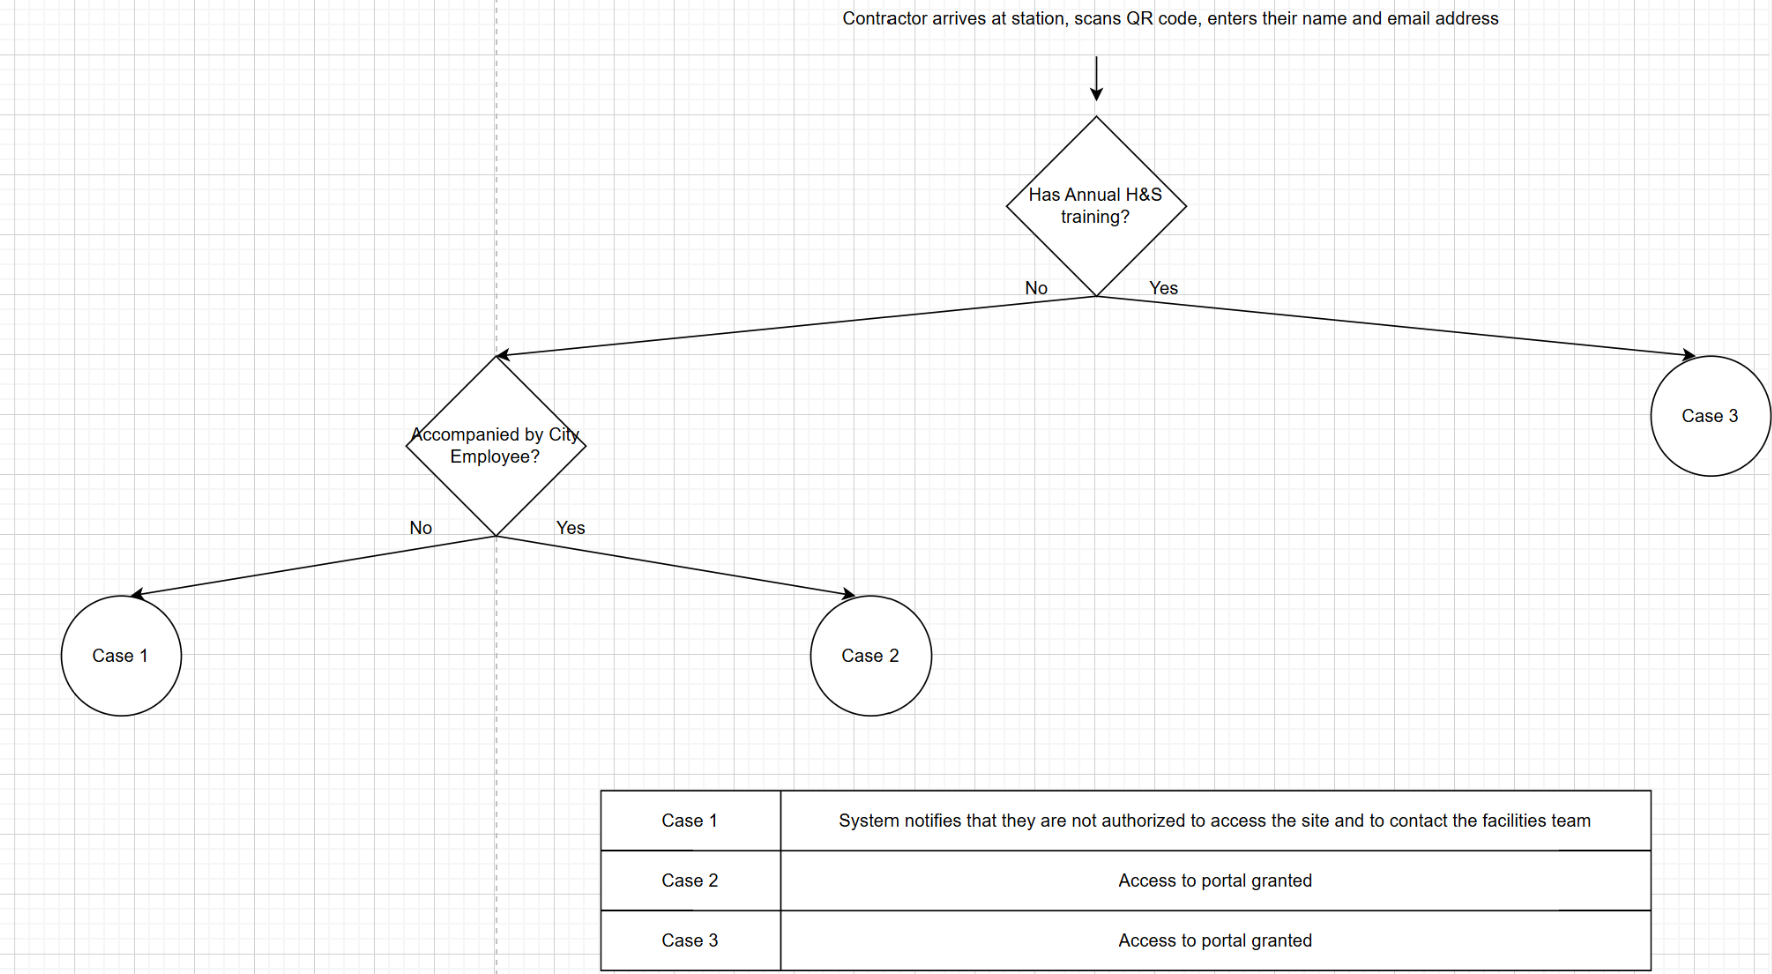
\includegraphics[scale=0.7]{ease_of_access.png}
  \caption{Prioritizing ease of access to the application with a
  visitor account}
\end{figure}
\newpage
\begin{figure}[h!]
  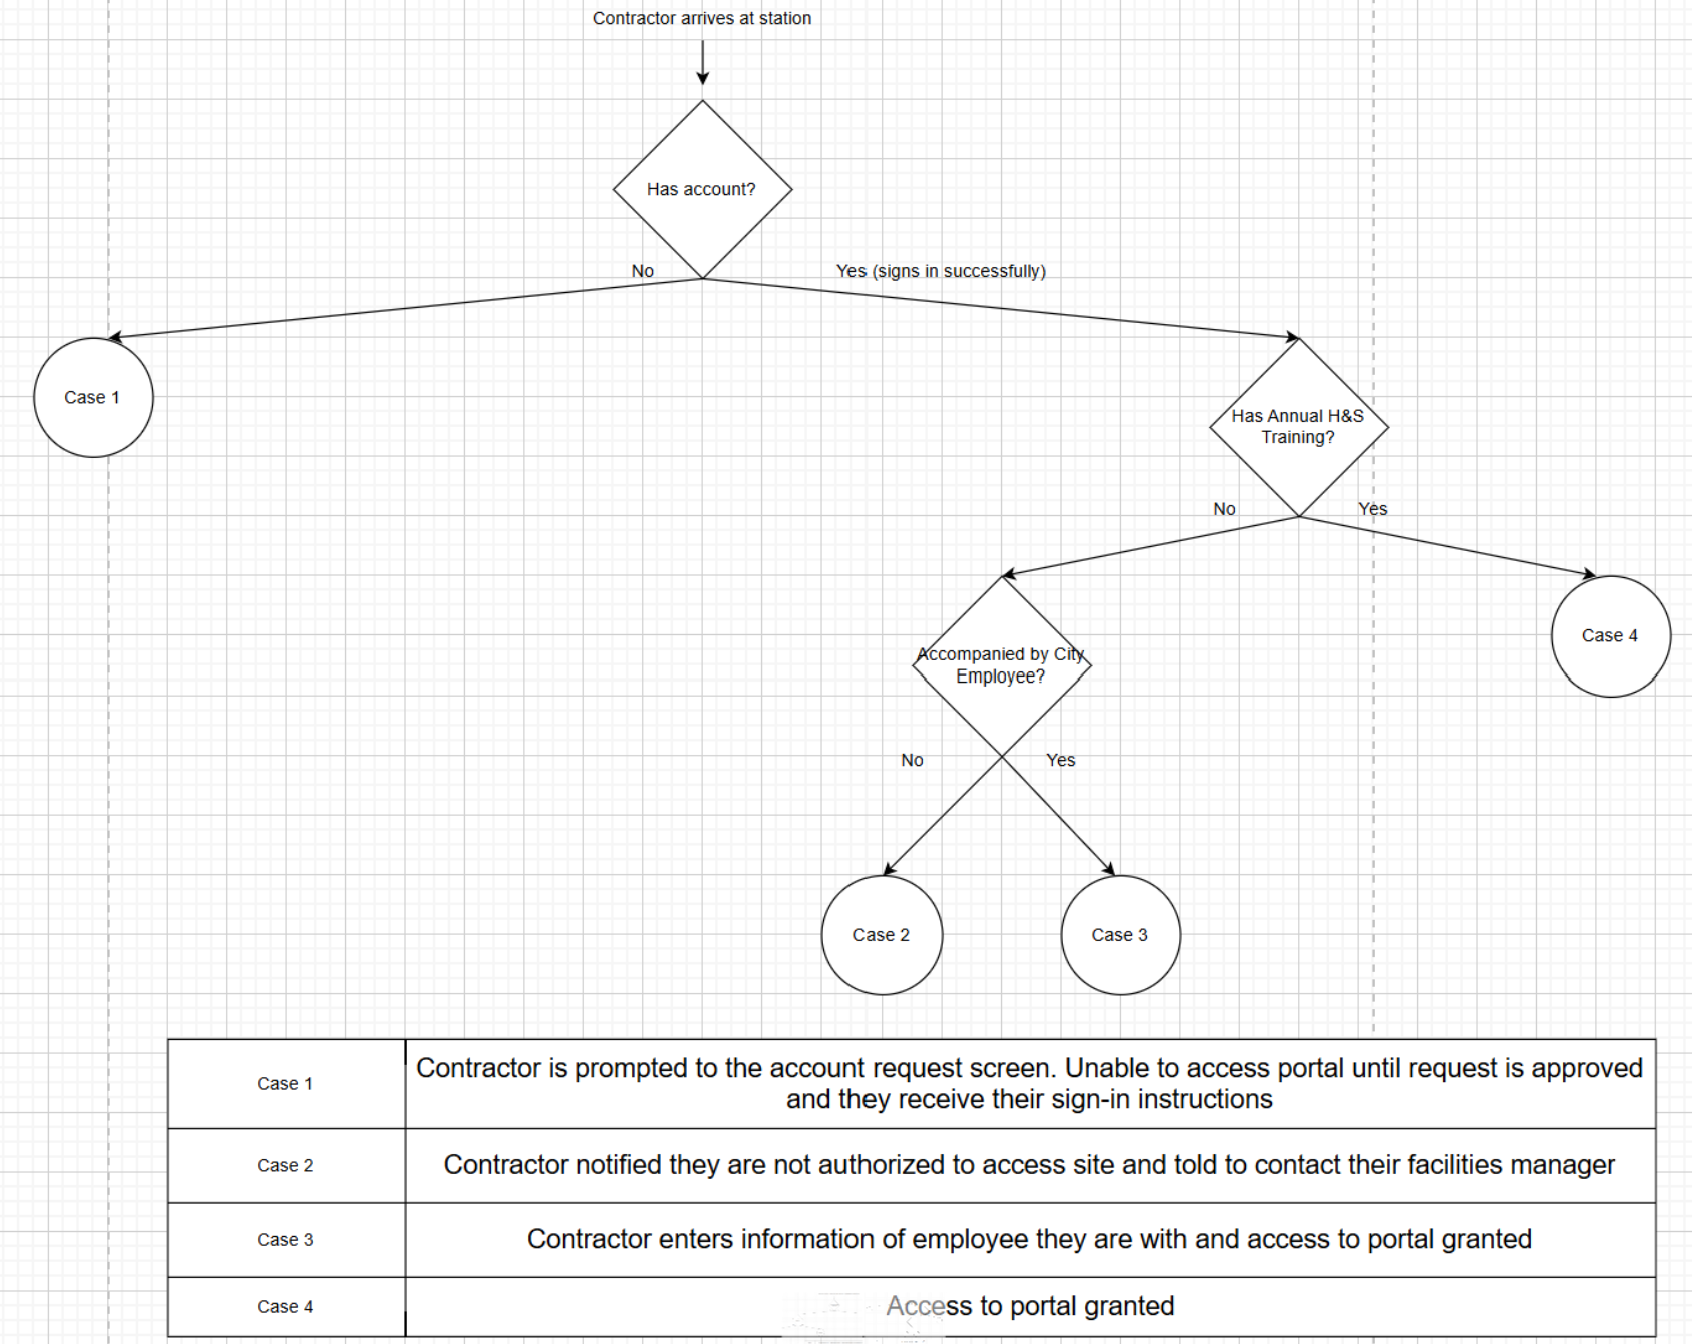
\includegraphics[scale=0.7]{trusted_access.png}
  \caption{Prioritizing security of the application
  by requiring a contractor account first be verified}
\end{figure}
\newpage
\section{Automated Testing}
N/A, the only automated testing we have is the unit tests.

\section{Trace to Requirements}

SRS \cite{SRS}

\begin{longtable}{|l|l|}
  \hline
  \textbf{Req. ID} & \textbf{Test ID's} \\
  \hline
  FR1 & TC-FR1, TC-FR2, UT-DM1\\ \hline
  FR3 & TC-FR3, UT-UM3\\ \hline
  FR4 & TC-FR4, UT-LG7\\ \hline
  FR5 & TC-FR5, UT-UA2\\ \hline
  FR6 & TC-FR6, UT-DM1\\ \hline
  FR7 & TC-FR8, UT-DM4, UT-DM6\\ \hline
  FR8 & TC-FR7, UT-LG1\\ \hline
  \sout{FR9} & \sout{TC-FR9}\\ \hline
  LF-AP1 & TC-LF-1 \\ \hline
  LF-ST1 & TC-LF-2 \\ \hline
  UH-EU1 & TC-EU1\\ \hline
  UH-EU2 & TC-EU2\\ \hline
  UH-LR1 & TC-LR1\\ \hline
  UH-LR2 & TC-LR2\\ \hline
  UH-UP1 & TC-UP1\\ \hline
  UH-UP2 & TC-UP2\\ \hline
  UH-AS1 & TC-AS1\\ \hline
  PR-SL1 & TC-PR-1\\ \hline
  PR-SL3 & TC-PR-2\\ \hline
  PR-SC1 & TC-PR-3\\ \hline
  PR-SC2 & TC-PR-4\\ \hline
  PR-PA1 & TC-PR-5\\ \hline
  PR-RFT1 & TC-PR-7\\ \hline
  PR-CR2 & TC-PR-10\\ \hline
  PR-SE1 & TC-PR-11\\ \hline
  OE-PE1 & TC-OE-1 \\ \hline
  OE-WE1 & TC-OE-2 \\ \hline
  OE-WE2 & TC-OE-2 \\ \hline
  OE-REL1 & TC-OE-4 \\ \hline
  OE-REL2 & TC-OE-4 \\ \hline
  OE-REL3 & TC-OE-4 \\ \hline
  OE-REL4 & TC-OE-4 \\ \hline
  MS-MTN4 & TC-MS-4 \\ \hline
  MS-MTN5 & TC-MS-11\\ \hline
  MS-MTN6 & TC-MS-6 \\ \hline
  MS-MTN7 & TC-MS-5 \\ \hline
  MS-SUP1 & TC-MS-7 \\ \hline
  MS-SUP2 & TC-MS-8 \\ \hline
  MS-SUP3 & TC-MS-9 \\ \hline
  MS-SUP4 & TC-MS-10 \\ \hline
  MS-ADP1 & TC-LF-2 \\ \hline
  MS-ADP2 & TC-LF-2 \\ \hline
  MS-ADP3 & TC-LF-2 \\ \hline
  SR-AR1 & TC-SS-1 \\ \hline
  SR-AR2 & TC-SS-1 \\ \hline
  SR-AR3 & TC-SS-1 \\ \hline
  SR-AR4 & TC-SS-2 \\ \hline
  SR-IR1 & TC-SS-2 \\ \hline
  SR-IR3 & TC-SS-4 \\ \hline
  SR-PR1 & TC-SS-5\\ \hline
  SR-AU1 & TC-SS-6 \\ \hline
  SR-IMR1 & TC-SS-7 \\ \hline
  SR-S1 & TC-SS-8 \\ \hline
  CR-CR1 & TC-CR-1 \\ \hline
  \caption{Requirements to Test Case Traceability Matrix}
\end{longtable}

\section{Trace to Modules}

MG \cite{MG},
MIS \cite{MIS}

Note: * indicates that any test prefixed with the test case ID,
covers the given module

\begin{longtable}{|m{5cm}|m{9cm}|}
  \hline
  \textbf{Module} & \textbf{Test ID's} \\
  \hline
  Database Interaction & UT-DB* TC-FR-1 TC-FR-2 TC-FR-8 TC-FR-7 TC-FR-6\\ \hline
  Logging & UT-LG* TC-FR-5 TC-EU1 TC-EU2\\ \hline
  File Storage & UT-FS* TC-FR-1 TC-FR-2 TC-PR-10 TC-PR-11\\ \hline
  Location Verification & UT-LV* TC-FR-5 TC-FR-8\\ \hline
  User Management & UT-UM* TC-FR-4 TC-FR-7 TC-SS-1 TC-SS-4 TC-PR-5
  TC-LR1 TC-LR2 TC-OE1 TC-OE2 UT-UR* \\ \hline
  User Authentication & UT-AU* TC-FR-9 TC-PR-4 TC-AS1 TC-LF1 TC-LF2
  TC-CR1\\ \hline
  Document Management & UT-DM* TC-FR-1 TC-FR-2 TC-FR-3 TC-FR-7
  TC-SS-2 TC-PR-1 TC-PR-3 TC-PR-5 TC-UP1 TC-UP2\\ \hline
  Site Management & UT-SM*\\ \hline
  \caption{Module to Test Case Traceability Matrix}
\end{longtable}

\section{Code Coverage Metrics}

The unit testing achieves 95\% line coverage and 90\% branch
coverage. This is checked by our GitHub Actions on every pull request.

\bibliographystyle{plainnat}
\bibliography{../../refs/References}

\newpage{}
\section*{Appendix --- Reflection}

The information in this section will be used to evaluate the team members on the
graduate attribute of Reflection.

The purpose of reflection questions is to give you a chance to assess your own
learning and that of your group as a whole, and to find ways to improve in the
future. Reflection is an important part of the learning process.  Reflection is
also an essential component of a successful software development process.  

Reflections are most interesting and useful when they're honest, even if the
stories they tell are imperfect. You will be marked based on your depth of
thought and analysis, and not based on the content of the reflections
themselves. Thus, for full marks we encourage you to answer openly and honestly
and to avoid simply writing ``what you think the evaluator wants to hear.''

Please answer the following questions.  Some questions can be answered on the
team level, but where appropriate, each team member should write their own
response:


\begin{enumerate}
  \item What went well while writing this deliverable?\\
    \\
    Our team did a reasonable job at allocating work based on
    everyones different skill sets. Team members with more experience in
    developing backend tools were responsible for the testing on
    those technologies, whereas team members more familiar with the frontend
    and business logic worked on testing those functionalities.
  \item What pain points did you experience during this deliverable, and how
    did you resolve them?\\
    \\
    One pain point we experienced was some complications fully
    implementing some of the more complex requirements and API integrations.
    This made it more difficult to test some aspects of the project
    and gave a tighter time frame. To resolve this, we used the Github
    issues to track progress on various components of the application
    and maintained regular communication to ensure we could
    be as prepared as possible for team meetings, meetings with the
    school, and meetings with the stakeholder.
  \item Which parts of this document stemmed from speaking to your client(s) or
    a proxy (e.g. your peers)? Which ones were not, and why?\\
    \\
    The parts of the document in sections 3 and 4 (functional and
    non-functional requirements) generally stemmed from conversation
    with our stakeholder. Those parts of the document are directly
    intended to ensure that the requirements gathered throughout the project
    are satisfied. Our stakeholder is relying on our knowledge for
    the actual implementation, so the specific unit tests and other technical
    decisions regarding the modules themselves were a decision made by our team.
  \item In what ways was the Verification and Validation (VnV) Plan different
    from the activities that were actually conducted for VnV?  If there were
    differences, what changes required the modification in the plan?  Why did
    these changes occur?  Would you be able to anticipate these
    changes in future
    projects?  If there weren't any differences, how was your team
    able to clearly
    predict a feasible amount of effort and the right tasks needed to build the
    evidence that demonstrates the required quality?  (It is expected that most
    teams will have had to deviate from their original VnV Plan.)\\
    \\
    There were some changes to the number of tests performed, these
    are reflected in the VnV Plan with strikeouts and red text
    to make clear which changes were made to the original plan. In
    general, for industry projects such as these,
    there is always going to be some unanticipated requirements or
    challenges not originally envisioned until you get into the depths
    of an implementation which then requires you to reevaluate either
    the requirements or your initial design. This was an expected
    challenge and we did our best to minimize the occurences, and in
    general there were not an enormous number of deviations.
\end{enumerate}

\end{document}
